\documentclass[journal]{IEEEtran}
\usepackage{amsmath}
\usepackage{fancyvrb}


% *** CITATION PACKAGES ***
%
\usepackage{cite}


% *** GRAPHICS RELATED PACKAGES ***
%
\ifCLASSINFOpdf
  \usepackage[pdftex]{graphicx}
\else
\fi


% correct bad hyphenation here
\hyphenation{op-tical net-works semi-conduc-tor}


\begin{document}
\title{Developing a Parallel Raster Plugin\\For QGIS}

\author{Alex~Feurst,
        William~Hoffman,
        Charles~Kazer,
        and~Dr.~Arthur~Lembo}%

\maketitle

% As a general rule, do not put math, special symbols or citations
% in the abstract or keywords.
\begin{abstract}
    Geographic Information Systems (GIS) are used in many different fields
    to analyze spatial data and plan accordingly. Geographic data has been
    growing in size exponentially, and while some GIS tools to analyze this
    data have been created, usage and efficiency have been lagging behind. The
    advent of massively parallel computing, specifically the availability of
    GPU programming, have made a more efficient solution possible since most
    GIS calculations are embarrassingly parallel. QGIS is an open source GIS
    platform that has gained much traction in the computational geography
    community. We created a QGIS plugin that leverages GPUs to increase
    calculation speed on large data sets. We developed this plugin with
    the geography community in mind, using Python to make code easy to read,
    portable, and modifiable.
\end{abstract}

\begin{IEEEkeywords}
    CUDA, Parallel Processing, GIS
\end{IEEEkeywords}



\IEEEpeerreviewmaketitle


\section{Background and Introduction}
\IEEEPARstart{W}{e} are three undergraduates from across the country that came
together in a National Science Foundation Research for Undergraduates for an 
educational experience in professional style research. Dr. Lembo came up with
the project that the three of us researched. Parallel computing has been adopted
in many fields to improve computation efficiency. Although many analytics in 
Geographic Information Systems (GIS) are embarrassingly parallelizable, 
parallel computing has yet to be largely adopted in the community. We've 
developed open source software for parallel raster calculations to spur the GIS
community to adopt parallel computing practices. This plugin was built for the
popular, open source GIS software QGIS, and performs parallel slope, aspect 
and/or hillshade calculations on an arbitrary raster file.  We've implemented 
the plugin using Python and PyCUDA, an open source library for Python built on 
top of the CUDA programming language for \textsc{NVIDIA} graphics cards. Our
current results indicate a efficient, scalable improvement over similar serial
calculations.

\section{Related Work} \label{related}
The idea of using parallel processing in GIS had been around for a long time
\cite{healy}, but only recently has been seriously considered.  Similar work on
creating open source, accessible parallel GIS tools has been done in the past,
though no one method has been widely adopted. The authors of \cite{Guan}
created a C++ library for parallel raster file processing, though this only
uses CPU parallelization. \cite{benedicic} created a GRASS GIS module based on
cluster computing designed to predict radio-coverage. \cite{Cheng} used 
parallelism to try and improve the computing i/o for digital terrain analysis.
GIS algorithms have also been parallelized over clusters of machines rather
than just CPU parallelization, such as in Huang\cite{huang}.  \cite{hpc_cuda} 
developed a C++ library for simple raster calculations using CUDA as an 
extension to the proprietary ArcGIS software. Implementation with CUDA and
GPUs was extended upon in \cite{Xu} to test the efficiency of a string
matching algorithm. GPUs and CUDA were also used in \cite{Saha} to apply
brightening and darkening filters. Other members of the computer science 
community in recent years have started testing methods to speed up the 
computing process on large scale data and some have used GPUs as well. 
\cite{Gaurav} tested a varity of GPU calculation methods and speed comparisons 
between all of them for future projects. GPUs were used on large scale pixel 
data in \cite{Wadbro} to show the usfulness of GPUs on big data. \cite{Zhang} 
used GPUs with grids of raster data to do speed comparisons with 
traditional search methods done on the CPU vs the GPU. Another highly 
repetative process was tested in% \cite{Yang} and \cite{Martínez-Frutos} 
with the testing of Sliding Windows Operations over CPUs and GPUs for 
compariaon. GPUs were used in comparison with Intel's Many Integrated Core
from \cite{Shi} to predict better efficiency for future spatial data 
problems. Large scale Digital Elevation Models were used in \cite{Tabik} by 
using solar measurements and angle data through a CPU-GPU heterogeneous 
system. We want to progress the work of these works to be more accessible 
to the GIS community.

\section{Problem Outline} \label{problem}
    \subsection{Computational Challenges}
    GIS analytics perform many independent calculations on extremely large data
    sets. This proves problematic due to the memory limitations of a single
    machine, and the massive amount of calculations that need to be run. Data sets 
    typically analyzed by GIS can be in the terabyte (TB) realm. With
    most computers only having memory capabilities in the gigabyte (GB) range,
    steps must be taken to work around running out of memory. Both the large size
    of data sets and the requirement that each piece of data be analyzed separately
    slows down processing time dramatically. Input from and output to data sets
    and memory have proven to be a major component to the slow down.  However,
    performing the large amount of independent calculations through serial
    programming also bogs down the process. Our goal is to build a system that
    maximizes Input/Output (I/O) throughput as well as reduce computation time
    through parallelism.

    \subsection{Ease of Use}
    Use of parallelism in GIS has been explored in the past, yet despite its proven
    benefits over serial calculation, the GIS community has been slow to adopt
    parallel computation. This is largely because the introduction of parallelism
    makes code much more difficult to read and write. Parallelism is something that
    many experienced programmers struggle with, let alone the many members of the
    GIS community who have little to no experience with programming. With this in
    mind, we have tried to write the parallel processing tools presented here in a
    simple, easy to modify way without giving up the power of parallelism
    altogether.  For those who don't even want exposure to any source code, we
    have provided a plugin to the popular, open source GIS, QGIS with a simple
    GUI that runs the parallel code.


\section{Methods} \label{methods}
    \begin{figure}
        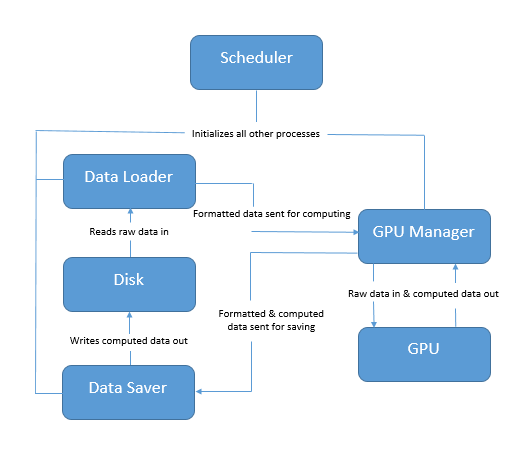
\includegraphics[width=\linewidth]{Model2.png}
        \caption{Main work flow model.}
        \label{model}
    \end{figure}
    \subsection{Scheduler Model}
    The previous work done in \cite{hpc_cuda} revealed that the greatest
    hindrance to performance in GPU based GIS calculations is the transfer of
    data from disk to main memory, and then from main memory to GPU memory.
    Memory transfer must occur four times for each GPU job, loading from disk
    to main memory, loading from main memory to GPU memory, and then copying
    results from GPU memory back to main memory, and then to disk.  Further
    compounding the problem is that GPU memory is typically more limited than
    main memory, so multiple copies from main memory are required for files
    larger than the available memory on the GPU. Thus we have designed our
    work flow to try to mitigate the effects of the I/O bottleneck.

    Figure \ref{model} shows our design model. There are three main processes,
    the data loader, the data saver, and GPU manager. Broadly, the data loader
    is responsible for loading data from disk and formatting from its initial
    file type, the data saver is responsible for compressing and saving data
    back to disk, and the GPU manager is responsible for running GPU tasks,
    including copying data to and back from the GPU. The three processes are
    described in more detail in section \ref{implementation}. The three
    processes run independently, so data can be loaded from disk, calculations
    can be performed on the GPU, and data can be saved to disk all
    simultaneously.  This provides parallelism both on the CPU for I/O, and on
    the GPU for calculations, improving overall computation time.
    
    \subsection{GPU Kernel}
    The GPU kernel, the algorithm that is executed on the GPU in parallel, is
    designed to perform analysis on individual cells in a raster file based on
    a 3x3 grid around the cell. The kernel was designed to be modular so that
    any kind of calculation can be done based on the 3x3 grid of neighbors. A
    user simply needs to write the desired calculation, and the rest of the
    kernel was written ensure that all of the correct data is available on any
    given thread for a 3x3 grid calculation.  The kernel uses a grid striding
    loop for flexibility and
    efficiency\cite{grid_stride}.

    \subsection{GIS Algorithms}
    The algorithms we implemented utilize a 3x3 cell neighborhood around each 
    calculated cell. 
    \begin{figure}
        \center
        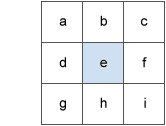
\includegraphics[width=2in]{GISgrid.jpg}
        \caption{3x3 cell neighborhood}
        \label{GIS grid}
    \end{figure}
    This 3x3 grid is used to calculate the rate of change from east to west
    \(\frac{dz}{dx}\) and the rate of change from north to south
    \(\frac{dz}{dy}\). These are found as follows:
    \[\frac{dz}{dx} = ((c + 2f + i) - (a + 2d + g) / (8 * x\_cellsize)\]
    \[\frac{dz}{dy} = ((g + 2h + i) - (a + 2b + c)) / ( 8 * y\_cellsize)\]
    where the letters correspond to the positions in \ref{GIS grid}.

    These rates of change are used to calculate slope, aspect and hillshade.
    Slope is the maximum rate of change in elevation between the cell and its
    neighbors. The lower the slope value the flatter the land is. It is
    calculated with the following formula:
    \[Slope = ATAN\Bigg(\sqrt{\Big(\frac{dz}{dx}\Big)^{2} + \Big(\frac{dz}{dy}\Big)^{2}}~\Bigg)\]

    Aspect identies the direction of the downslope. Aspect is found using
    %conditional steps and is calculated in degrees, which can be converted to
    %radians.
    the following formula:
    \[Aspect = 57.29578 * ATAN2\bigg(\frac{dz}{dy}, -\frac{dz}{dx}\bigg)\]

    Hillshade is the hypothetical illumination of the surface when the sun is
    at a specific height and angle in the sky. It is a more complex algorithm
    and relies on slope and aspect being calculated in addition to finding the
    illumination angle zenith (abbreviated \(zen\)) and illumination
    direction azimuth (abbreviated \(azm\)). We have defaulted these values
    to 45 degrees and 315 degrees respectively.
    \begin{align*}
        Hillshade =& ~ 255.0 ((COS(zen) * COS(slope)) ~ +  \\
                   &(SIN(zen) * SIN(slope) * COS(azm - aspect))
    \end{align*}

    \subsection{QGIS Integration}
    We have constructed a QGIS plugin, depicted in figure \ref{gui} which uses
    our data processing pipeline and presents a simple GUI where a user can
    select an input file, output file, and operations to perform. This way,
    once the plugin is installed, a user need not even interact with the
    command line, or learn to use a new piece of software in order to perform
    GPU calculations. We have also tried to allow users to load data directly
    from QGIS rather than from disk, but this feature is still unstable.
    \begin{figure}
        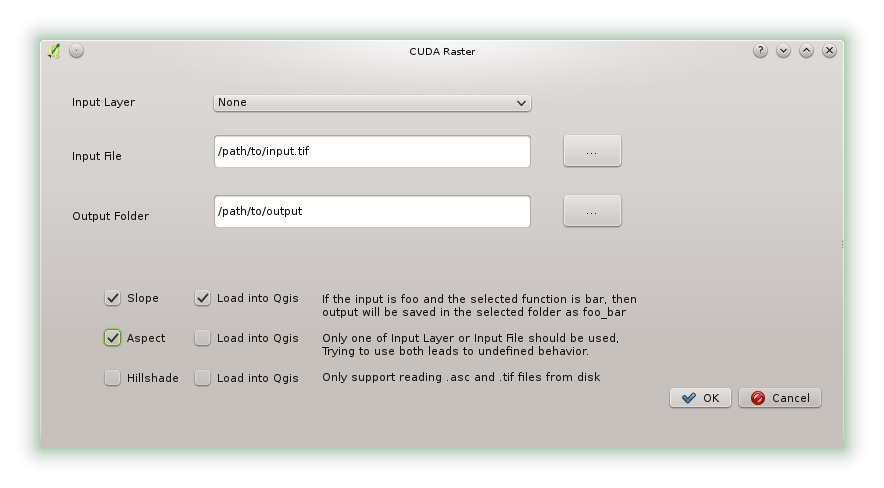
\includegraphics[width=\linewidth]{gui.png}
        \caption{Snapshot of plugin GUI.}
        \label{gui}
    \end{figure}

\section{Implementation} \label{implementation}
    Our program is implemented primarily in Python 2.7. We chose to write the
    program in Python because it is relatively easy to read and write, and also
    allowed us to produce shorter, more compact code than the C or C++ code
    typically used with CUDA.  Although Python is slower than C or C++, we
    thought the readability trade-off was worth it so that others in the GIS
    community could read, test, and modify our code. In order to still get as
    much efficiency as possible, we used the GDAL libraries, Numpy, and PyCUDA
    \cite{pycuda_1} \cite{pycuda_2}. PyCUDA serves as a wrapper for CUDA C that
    handles many of the ugly details of memory allocation and transfer to the
    GPU. Unfortunately, kernel code to be executed on the GPU must still be
    written in C. 
    
    Our program's structure follows the model in figure \ref{model}. The
    following sections describe the implementation of each process.

    \subsection{Scheduler}
    The scheduler class starts and manages the other processes. It is
    responsible for parsing the desired input, functions, and output. It starts
    each other process and coordinates passing information between them. The
    scheduler also ensures that each other process terminates properly, and if
    not attempts to print useful information about which process caused the
    error. Although figure \ref{model} only depicts one saver, multiple
    functions can be computed on a single file loaded by the data loader, and
    the scheduler will generate a different saver to individually save each
    output.
    
\begin{Verbatim}[frame=single, gobble=4]
    Start DataLoader, GPUManager
       and DataSaver;
    While DataLoader, GPUManager 
       or DataSaver is active;
       if (DataLoader errors)
          Stop GPUManager 
          and DataSaver;
          Break while;
       end If
       If (GPUManager errors)
          Stop DataLoader 
          and DataSaver;
          Break while;
       End If
       Wait one second;
    End While
    Timer = timenow 
       - starttime;
    print timer;
\end{Verbatim}
    \break

    \subsection{Loader}
    The loader class reads data from a given input file and passes it into
    a pipe object, which goes to the GPU manager. We use the GDAL libraries to
    read files from disk because it is optimized on raster data files. The data is
    formatted row by row into Numpy arrays and then passed to the GPU manager.
    We chose to have a single row of data be our transfer unit because it makes
    both the loader and the GPU kernel easier to understand than if we tried to
    use two dimensional blocks of data. The loader class is also responsible
    for providing the GPU Manager and data saver file metadata, such as the
    dimensions of the raster and the area that each pixel represents.

    Originally, we pulled lines from the file with GDAL one by one, matching
    how we send one row at a time through the pipe. However, we found that this
    could be made more efficient if GDAL read more rows per read call, likely
    because fewer system calls are made that way. Empirically, the optimal number
    of rows to cache depends on the dimensions of the raster file. 30 rows seems
    to be a good starting point.

\begin{Verbatim}[frame=single, gobble=2]
  inputdata equals lines
     read from raster file;
  unpack inputdata into 
     blocks of data based on lines;
  For (blockdata in inputdata)
     send blockdata in rows 
        and columns to GPUManager;
  End For	
\end{Verbatim}

    The QGIS plugin version also supports reading raster data from a layer loaded
    into QGIS rather than from disk. When read this way, the loader uses the QGIS
    python API to load a Numpy array of a single row of data.

    \subsection{GPU Manager}
    The GPU manager is where the actual calculations on the data are performed,
    and where the bulk of the code exists. The manager functions by reading a
    page worth of data from the input pipe, performing GPU calculations on that
    page, then sending that through an output pipe to the data saver. Each page
    is sized to exactly fit a certain number of rows of data. The GPU manager
    is designed to be robust in that it bases all of its memory management on
    the GPU card of the system it runs on. Although the kernel code is somewhat
    complex, it is designed so that one could write any algorithm based on a
    3x3 grid of pixels to be plugged into the rest of the kernel code and calculated.

    The GPU manager starts by initializing the buffers which will be used to
    copy memory to and retrieve memory from the GPU. These are based on the
    available GPU memory when the process starts, so it should always saturate
    GPU memory. It then pre-compiles the GPU kernels for each requested
    calculation on the data. Finally, the manager enters the main processing loop
    where data is received and analyzed.

    Once the read buffer receives a page worth of data, it serially runs each
    requested kernel, copies the results back from the GPU, and sends the data
    for each kernel to a different saver. Each kernel is scheduled to run on
    as many GPU cores as possible, to minimize computation time.

\begin{Verbatim}[frame=single, gobble=8]
        Grid equals 256 by 256;
        Blocks equals 32 by 32 
           by 1;
        Blocks equals grid 
           position 0 times grid 
           position 1;
        Thread equals blocks 
           position 0 
           times blocks 
           position 1 
           times blocks 
           position 2;
      
        PixelsinThread equals 
           rows times columns 
           divided by numberofThreads 
           times numberofBlocks;
	 
        While (pixelsinThread less than 3)
            Newgrid equals grid 
               position 0 minus 16 by 
               grid position 1 by 16;
            Newblocks equals newgrid 
               position 0 times newgrid 
               position 1;
            NewpixelsinThread equals 
               rows times columns divided
               by numofThreads times 
               numofBlocks;
            pixelsinThread equals 
               numpy ceiling with pixelsinThread;
        End While
   
        struct equals GPU struct of
           numpyinteger64 by 
              pixelsinThread by pixelsinThread;
           numpyfloat64 by NODATA by NODATA;
           numpyinteger64 by numberofcolumns
              by column;
           numpyinteger64 by number 
              of rows by row;
           numpyinteger numberofPixels by 
              row times column;
           numpyfloat32 by cellsize by 
              cellsize;
        End Struct

        Copy struct into GPU;
        Function gets passed GPUdata and 
         GPUresult and struct and block and grid;
\end{Verbatim}

    \subsection{Saver}
    The data saver class takes the results of the calculations done in the GPU
    manager and saves them to disk. Similar to the data loader, the data saver
    uses the GDAL libraries to write multiple lines at a time to a Geotiff.
    Multiple savers can all run in parallel to save the ouputs of different
    functions.
\break
\begin{Verbatim}[frame=single, gobble=4]
    Try (code if no errors)
       For (row in the 
          numberofRows)
          numpy put in ouputarrayrow 
             and recievedinputpipe;
       END For
       If (end of file)
          print unexpected 
             end of file;
          Stop Everything;
       Enf If
    End Try
    Write results to output array 
       from position 0 to number of rows;
\end{Verbatim}


    \subsection{QGIS Plugin}
    For QGIS, we implemented a simple GUI plugin that calls our code. The plugin
    was made using the QGIS plugin builder tool to generate all of the skeleton
    code and QT creator to design the GUI. The plugin takes input and output
    information from the user, then calls the scheduler on those parameters.

    Although there are a still a few issues, we also implemented loading data
    from a QGIs layer, rather than from disk. This separate version of the loader
    reads values using the QGIS API, so if QGIS has raster information cached in
    memory, it should load values faster than from disk. The QGIS loader still
    sends one row of data at a time through a pipe, so no changes are needed
    for it to work with the GPU manager or data saver.

\begin{Verbatim}[frame=single, gobble=7]
       Currentlayer equals inputlayer;
       Size of layer equals inputlayersize;
       Data equals currentlayer data;
       Create empty array;
       For (element in range of layer width)
          Array appends with 
             row data element;
       End For
       Return array as float32; 
\end{Verbatim}
    
\section{Analysis}
Timing our implementation for parallel hillshade and slope calculation from a raster file
against the standard serial methods used in QGIS has revealed the input and
output will be our biggest hurdle to overcome. Timing data can be seen in these
tables.

\vspace{.25in}
\pagebreak
\textbf{Hillshade timings}
\vspace{0.05in}

\begin{tabular}{ l | c | c }
    File Size & QGIS   & PyCUDA\\ \hline
    25 MB     & 5 secs & 3 secs\\ \hline
    200 Mb    & 15 secs & 6 secs\\ \hline
    1.5 GB    & 11 mins & 3 mins\\ \hline
    8 GB      & 45 mins & 30 mins
\end {tabular}

\vspace{.25in}
\textbf{Slope breakdown}
\vspace{0.05in}

\begin{tabular}{ l | c | c }
    Function    & QGIS & PyCUDA\\ \hline
    Input       & 2:00 & 1:55\\ \hline
    Computation & 5:00 & 1:00\\ \hline
    Output      & 2:00 & 2:20\\ \hline
    Total       & 9:00 & 3:35
\end {tabular}

\vspace{.25in}
\textbf{Hillshade breakdown}
\vspace{0.05in}

\begin{tabular}{ l | c | c }
    Function    & QGIS & PyCUDA\\ \hline
    Input       & 2:00 & 1:55\\ \hline
    Computation & 7:00 & 1:00\\ \hline
    Output      & 2:00 & 2:20\\ \hline
    Total       & 11:00 & 3:35
\end {tabular}
\vspace{0.25in}

The PyCUDA version is consistently faster than QGIS when calculating hillshade
for files of various sizes. The I/O bottleneck  can be seen in the input and
output sections of the second table. PyCUDA spends almost as much time dealing
with disk as QGIS does which limits the maximum speedup from using the GPU.
Output takes a much longer time because it has to wait for the GPU to pass data
to the saver before it can start saving to disk.  GPU computations, including
CPU based memory management took one ninth of the time required to do the
same thing in QGIS. Most of this time is spent sending or receiving data, once
the information is on the card the GPU finishes extremely quickly. Including
moving data to and from the card, the accumulated execution time for the GPU
was less than 2 seconds.  Both slope and hillshade are calculated in almost the
same time by the GPU, showing that it isn't being significantly taxed by the
more complicated formula and could easily do more work.  A process that
required hundreds or thousands of computations per element would be perfect for
adaptation onto GPU processing. Testing showed that even computing hillshade
several hundred times on each pixel didn't increase the time needed to finish.


\section{Conclusion}
We have developed a PyCUDA based, open source raster calculation tool that can
run either from the command line or as a plugin for QGIS. The plugin ensures
that neither memory on the host device or GPU will be overpopulated, and
utilizes multiprocessing so that I/O and GPU computation can occur
simultaneously. The underlying code was written to be easy to read and modify
so that others can easily use it, read it, learn from it, and modify it. File
I/O is encapsulated separately from GPU calculations so that the I/O model is
easy to understand and modify. By default, our tool can perform slope, aspect,
and hillshade calculations. Our results show that our raster calculation
implementations are 3-5x faster than the serial ones typically used by QGIS, and
that the performance gap widens for larger files and more complex calculations.
The greatest bottleneck in our program is data I/O transfer between the disk,
main memory, and GPU memory, as even for files in the tens of GB, GPU
calculations take only a handful of seconds.  Hence, anyone who designs a more
complex function to run with our kernel can expect to see even greater time
savings over a serial implementation. Additionally, we designed a simple to use
GUI for the plugin so that even those with no coding experience can still use
the tool.This was a great educational experience for the three of us as we 
venture into our future endevures in grad school and the professional world.

\section{Future Work}
Many more GIS problems could be analyzed using massively parallel GPU
computation.  Our tool only allows for independent raster computations based on
a 3x3 grid around a given cell, however, with relatively little change, this
could be extended to larger grids, like 5x5 or greater.  The GPU could also be
used to different kinds of computation altogether with multiple kernels, such
as analysis on raster data where each computation may have dependency on
another, or even analysis on vector data.

The plugin currently has minimal integration with QGIS. Aside from being able
to load data using the QGIS API, the plugin is just a wrapper for the tool
that reads from and writes to disk. Further integration with QGIS could improve
both performance and usability of the plugin.

Currently, the slowest part of the computations by and far is file I/O. Further
optimizing I/O and exploring new I/O methods and/or models could significantly
improve run time. While our model supports asynchronous I/O and computation to
some extent, in reality the vast majority of the time the GPU isn't utilized
while it is waiting for data to be loaded. However, using faster methods to
improve I/O may lead to more complex code that is more difficult to read,
write, debug, and modify, so this trade off must be considered if one desires
their code to be easily usable in the open source community.

\ifCLASSOPTIONcaptionsoff
  \newpage
\fi

\bibliographystyle{IEEEtran}
\bibliography{references}
\end{document}
